\section{Introduction}
Most path planning studies have been focused in one of two directions: identifying better heuristics to 
guide search and reducing the search space through hierarchical decomposition.
In the case of the former, it has been shown that even almost perfect heuristics can result in poor 
performance \cite{malte08,korf98}. 
In the case of the latter, the search space is reduced but optimality is not preserved. 
It seems then that the reduction of search spaces while preserving optimality, as we do in this work, is a good direction for research.
\par
We begin by considering the problem of optimal path planning on 4-connected grid maps (or tile maps),
so called because movement is restricted to the four cardinal directions, 
This simple domain appears in application areas such as robotics \cite{latombe91} and video games 
(cite one of the Game/AI Programming Gems books).
Although not as popular as 8-connected octile grid maps (which allow diagonal transitions) the 4-connected case has 
the advantage of producing many highly symmetrical paths; 
a property we exploit in order to derive the main result of this paper.
\par 
Our work is motivated by the seemingly innocuous problem in Figure \ref{fig-emptymap} 
which requires finding a shortest path from S to G in a mostly empty room.
\begin{figure}[htbp]
HPA* \cite{botea04} proceeds by dividing a grid map into a series of fixed-size clusters connected 
by entrances.
	\vspace{-4pt}
       \begin{center}
                       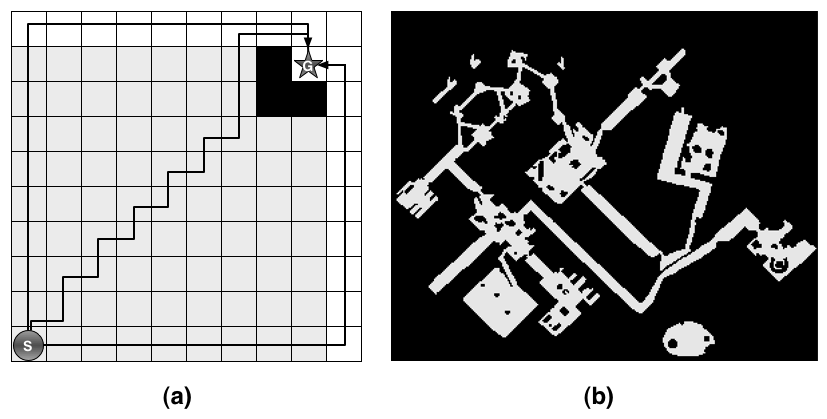
\includegraphics[scale=0.30, trim = 20mm 20mm 20mm 0mm]{diagrams/emptymap.png}
       \end{center}
	\vspace{-3pt}
       \caption{\textbf{(a)} A simple (yet computationally difficult) pathfinding problem; find an 
optimal length path from $S$ to $G$ in a mostly empty area. 
Many solutions exist; we highlight three. 
\textbf{(b)} A typical map from BioWare's Baldur's Gate.}
       \label{fig-emptymap}
	\vspace{-12pt}
\end{figure}
This scenario appears as a subproblem in many real-world path planning applications but particularly
in video games.
For example, BioWare's popular fantasy role-playing game \emph{Baldur's Gate} features complex dungeon
 areas that are composed of adjacent mostly empty rooms (see Figure \ref{fig-emptymap}(b) for an example).
If we apply A* \cite{hart68} to solving the instance in Figure \ref{fig-emptymap}, using an almost 
perfectly informed manhattan heuristic, we find that the algorithm must expand all tiles in the grey 
area and at least some of those in the white area.
Given an unfavourable tie-breaking strategy A* will generate all nodes on the map and of those expand 
all but one.
\par
In solving the problem from Figure \ref{fig-emptymap} it is helpful to observe that although many optimal 
length solutions exist all are dominated by the two paths which may be found along the perimeter of 
the room. 
We generalise this observation to the related problem of traversing across empty rooms (which are 
often just as difficult for A* to solve) and show that it is possible to optimally navigate across 
such areas without ever exploring tiles that are not on the perimeter.
This result forms the basis for a new hierarchical search method which decomposes 4-connected grid maps
into a set of adjacent empty rooms. 
We undertake an empirical analysis and show that our technique retains the optimality guarantees of A* 
yet performs similarly to a state-of-the-art hierarchical planner which is memory-efficient but suboptimal.
